\section{Introduzione ai grafi}

\subsection{Grafi}

Un grafo $G$ è costituito da una coppia di insiemi $(V, A)$ dove:
\begin{itemize}
    \item $V$ è l'insieme dei \textbf{nodi}
    \item $A$ è l'insieme degli \textbf{archi}
\end{itemize}

Il grafo può essere \textbf{orientato} o \textbf{non orientato}, si capisce dalle frecce presenti sulgi archi.

I grafi sono oggeti matematiche con i quali è possibile rappresentare in maniera astratta le relazioni fra le entità(nodi).

Se la relazione è simmetrica(cioè $i$ è in relazione con $j$ se e solo se $j$ è in relazione con $i$) gli archi 
usati saranno privi di orientamento.

\textbf{Esempio}:

\begin{itemize}
    \item la relazione "è padre di" non è simmetrica
    \item la relzione "è fratello di" è simmetrica
\end{itemize}

\textbf{Esempio}:

Avendo un grafico del tipo:

\begin{equation*}
    V = \{a, b, c, d, e\}
\end{equation*}

Se si parla di un grafo orientato, l'arco $(a, b)$ è diverso dall'arco $(b, a)$.

Se parliamo di grafi non orientati l'ordine di comparizione delle lettere dell'arco non ha nessun impatto.

\textbf{Definizione}:

Dato un grafo \textbf{orientato} $G = (V, A)$ e un arco $(i, j)$:
\begin{itemize}
    \item diremo che $i$ è \textbf{predecessore} del nodo $j$.
    \item diremo che $j$ è \textbf{successore} del nodo $i$.
\end{itemize}

Dato un grafo \textbf{non orientato} $G = (V, A)$ e un arco $(i, j)$:
\begin{itemize}
    \item diremo che $j$ e $i$ sono \textbf{adiacenti}.
\end{itemize}

\subsection{Liste di adiacenza}

Ogni nodo del grafo ha una lista dei suoi successori(grafo orientato) o dei suoi adiacenti(grafo non orientamento).
\begin{figure}[h!]
    \centering
    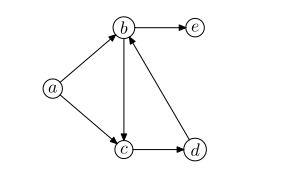
\includegraphics[width=0.4\linewidth]{img/Screenshot from 2022-05-31 15-50-09.png}
    \label{fig:example_graph}
    \caption{Esempio di grafo orientato}
\end{figure}

Le liste di adiacenza verrranno fuori a seconda dei tipi di grafo:

\subsubsection{Grafo orientato}
\begin{equation*}
    a: (b, c)\quad b: (c, e)\quad c: (d)\quad d: (b)\quad e: (\emptyset)
\end{equation*}
\subsubsection{Grafo non orientato}
\begin{equation*}
    a: (b, c)\quad b: (a, c, d, e)\quad c: (a, b, d)\quad d: (c, b)\quad e: (b)
\end{equation*}

\subsection{Matrice di incidenza nodo-arco}
Matrice con tante righe quanti sono i nodi e tante colonne quanti sono gli archi.

\subsubsection{Grafo orientato}
\begin{figure}[h!]
    \centering
    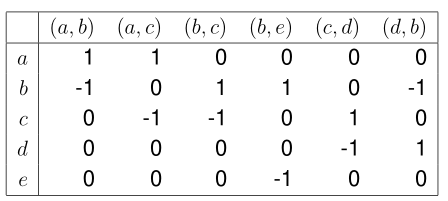
\includegraphics[width=0.5\linewidth]{img/Screenshot from 2022-05-31 16-13-04.png}
\end{figure}

\subsubsection{Grafo non orientato}
\begin{figure}[h!]
    \centering
    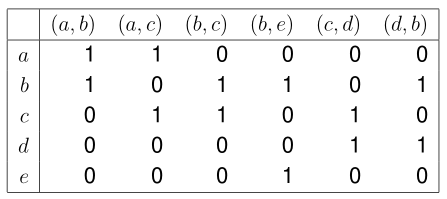
\includegraphics[width=0.5\linewidth]{img/Screenshot from 2022-05-31 16-14-15.png}
\end{figure}

\subsection{Archi adiacenti e cammini}
Due archi con un nodo in comune sono detti \textbf{adiacenti}.

Il cammino è il il percorso per arrivare da un nodo ad un'altro, e la lunghezza del cammino è il numero di archi.


Un cammino è detto \textbf{semplice} se nessun arco è percorso più di una volta,
\textbf{elementare} se nessun nodo viene toccato più di una volta.

\subsection{Cicli}
Se il primo e ultimo nodo di un cammino sono uguali, il cammino si chiama ciclo.

\subsubsection{Cammini e cicli orientati}
Se gli archi sono percorsi con il loro orientamento(siamo per forza in un grafo orientato), il ciclo si chiama
oreintato, altrimento non orientato.

\subsection{Circuiti Hamiltoniani}

Un circuito Hamiltoniano è un ciclo elementare che (orientato ne lcaso di un grafo orientato) che 
tocca tutti i nodi del grafo.

\subsection{Componenti connesse}
Dato un grafo, se posso andare da $i$ a $j$, si dice che $j$ è accessibile da $i$.

Un grafo si dice \textbf{connesso} se tutti i nodi sono accessibili tra di loro(il grafo ha un'unica componente connessa).

\subsection{Grafo completo}
Un grafo si dice completo se essite un'arco che congiunge 
ogni coppia di nodi distinti el grafo.

Se il grafo è orientato, devono essere presenti sia gli archi $(i, j)$ che gli archi $(j, i)$.

\subsection{Sottografi}
È un sottoinsieme degli archi dell'insieme di partenza

\textbf{Esempio}:


Grafo di partenza:

\begin{equation*}
    G = (V, A)
\end{equation*}

Se $A' \subseteq A$, 

\begin{equation*}
    G' = (V, A')
\end{equation*}
viene detto \textbf{grafo parziale} di G.

Se il grafo è viene creato fornendo un sottoinsieme dei nodi(al posto che archi):
\begin{equation*}
    A'' = A(V'')
\end{equation*}
Quindi il grafo sarà:
\begin{equation*}
    G'' = (V'', A'')
\end{equation*}

e si denota con: \textbf{sottografo indotto} dai vertici.

\subsection{Matching}
Dato un grafo $G = (V, A)$ non orientato, chiamiamo matching
un sottoinsieme $M \subseteq A$ dell'insieme di archi con la proprietà
che ogni nodo $i \in V$, esiste al massimo una arco $M$ avente come estremo il nodo $i$.

\subsection{Grafi bipartiti}
Un grafo $G = (V, A)$ si dice \textbf{bipartito} se l'insieme dei vertici(nodi o $V$)
può essere partizionato in due sottoinsiemi $V_1$ e $v_2$ dove:
\begin{itemize}
    \item $V_1 \cup V_2 = V$
    \item $V_1 \cap V_2 = \emptyset$
\end{itemize}

in modo che un vertice non compaia in entrambi i sottoinsiemi.

Se ogni coppia $i \in V_1, j \in V_2$ si ha che $(i, j) \in A$, allora il grafo si chiama \textbf{bipartito completo}.

\subsubsection{Riconoscimento grafi bipartiti}
\begin{enumerate}
    \item Pongo $W = V, C_1 = C_2 = \emptyset$
    \item Seleziono $i \in W$ e pongo $T_1 = \{i\}, c_1 = T_1$
    \item Pongo $T_2 = \{k \in V\backslash C_2 : \exists i \in T_1$ tale che $(i, k) \in A$ oppure $(k, i) \in A\}$, 
           \begin{itemize}
               \item  Pongo $C_2 = C_2 \cup T_2$
           \end{itemize}
    \item Pongo $T_1 = \{k \in V\backslash C_1 : \exists i \in T_1$ tale che $(i, k) \in A$ oppure $(k, i) \in A\}$, 
           \begin{itemize}
               \item Pongo $C_1 = C_1 \cup T_1$
           \end{itemize}
    \item Se $C_1 \cap C_2 \neq \emptyset$ allroa il grafo non è bipartito, altrimenti vado al passo 6.
    \item Pongo $W = W \backslash (C_1 \cup C_2)$
        \begin{itemize}
            \item se $W = \emptyset$ e $T_1 = \emptyset$, il grafo è bipartito con $V_1 = C_1$ e $V_2 = C_2$
            \item se $T_1 = \emptyset$, ritorno al passo 2
            \item Se $T_1 \neq \emptyset$, ritorno al passo 3
        \end{itemize}
\end{enumerate}

\subsection{Alberi}

Sia dato un grafo $G = (V, A)$ con cardinalità(numero di elementi): $card(V) = n$.

Si dice che $G$ è un'\textbf{albero} se soddisfa le seguenti condizioni(equivalenti tra loro):
\begin{itemize}
    \item $G$ è privo di cicli e connesso
    \item $G$ è privo di cicli e $card(A) = n - 1$
    \item $G$ è connesso e $card(A) = n - 1$
    \item Esiste un cammino elementare che congiunge tutti i nodi
\end{itemize}

\subsection{Alberi di supporto}

Sia definito un grafo generico $G = (V, A)$.

Si definisce \textbf{albero di supporto} o \textbf{spanning tree} di $G$ un grafo parziale 
$T = (V, A_T)$ dove $A_T \subseteq A$ che è un albero.

Un'albero di supporto deve contenere tutti i nodi, quindi si fa un sempling degli archi.

